\chapter{ALICE ad LHC}

\section{LHC}
A poca distanza da Ginevra si trova il più grande collisore di particelle del mondo: il \textit{Large Hadron Collider} (LHC). Questo acceleratore ha un raggio complessivo di 27~Km ed è stato costruito a partire dal 1998 dall'Organizzazione Europea per la Ricerca Nucleare (Cern) con lo scopo di progredire nella conoscenza dell'Universo e dei suoi meccanismi più profondi.
\\In figura \ref{fig:CERNcomplex} è mostrato il complesso di acceleratori del CERN, di cui LHC rappresenta l'ultimo stadio. L'insieme degli acceleratori \`e composto da un iniziale acceleratore lineare (Linac2), seguono tre sincrotroni, il Proton Synchrotron Booster (PSB), il Proton Synchrotron (PS) e il Super Proton Synchrotron (SPS), dal quale si ottengono particelle accelerate a 450~GeV, che vengono infine iniettate nell'LHC dove raggiungono un'energia di 6.5~TeV. 
 
    \begin{figure}[htbp]
        \centering
        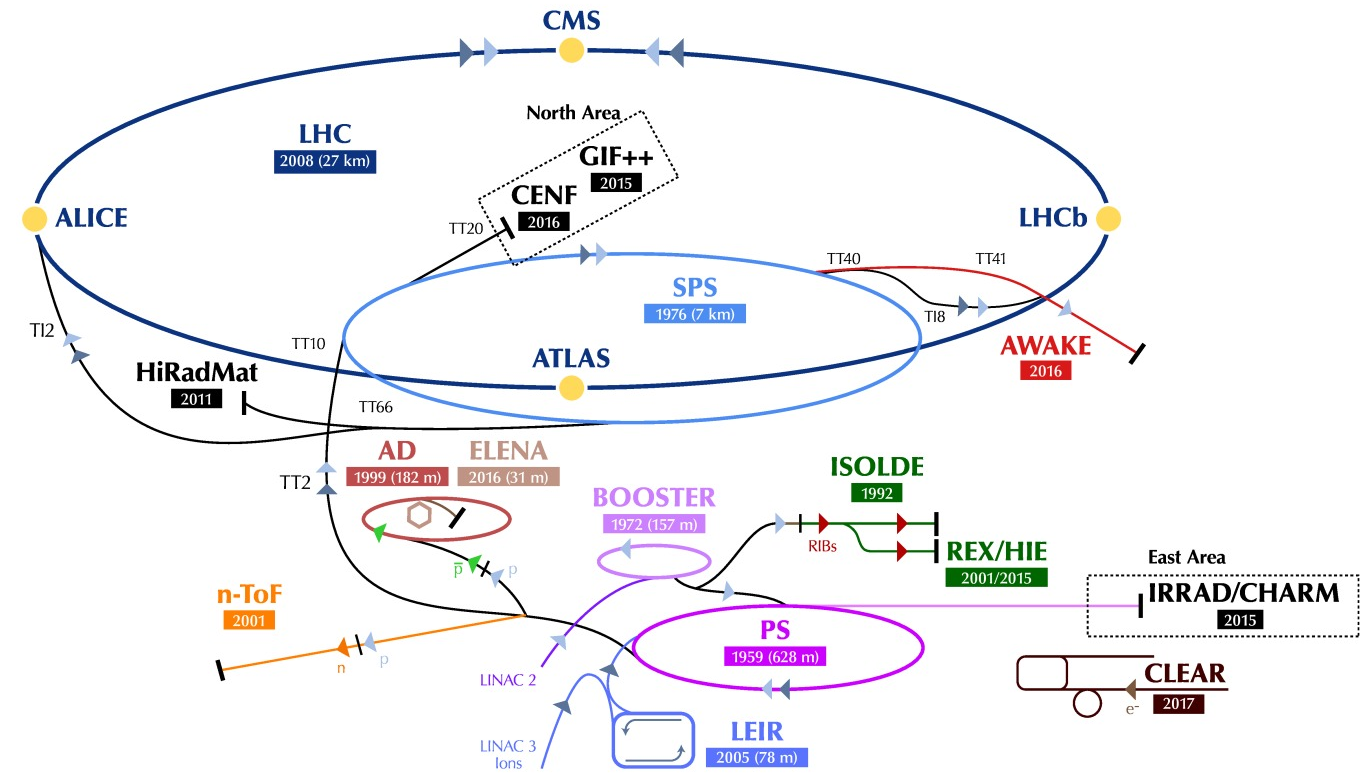
\includegraphics[width=0.8\linewidth]{ALICE/CernComplex_2018.png}   
        \caption{Complesso dell'intero acceleratore del CERN \\\small{Si vedono  \textcolor{blue}{LHC \textit{Large Hadron Collider}} \textcolor{cyan}{SPS \textit{Super Proton Synchrotron}} \textcolor{purple}{ PS \textit{Proton Synchrotron}} \textcolor{violet}{BOOSTER \textit{Proton Synchrotron Booster}} LINAC \textit{Linear ACcelerator}} \\{\footnotesize  \textcolor{red}{AD \textit{Antiprotron Decelerator}} \textcolor{green}{ISOLDE \textit{Isotope Separator Online DEvice}}  \textcolor{lightgray}{LEIR \textit{Low Energy Ion Ring}} }}
        \label{fig:CERNcomplex}
    \end{figure}
    
Il fascio di particelle viaggia in un tubo in cui viene fatto l'ultra-vuoto ed è direzionato da dei magneti superconduttivi tenuti alla temperatura di 1.85~K.

\section{ALICE}

L'acronimo ALICE sta per \textit{"A Large Ion Collider Experiment"} e lo  scopo primario dell'esperimento è quello di studiare la materia nucleare ad alte densità e alte temperature in uno stato chiamato \textit{Plasma di Quark e Gluoni} (QGP). Il QGP è caratterizzato da quark e gluoni liberi e non confinati negli adroni dalla forza nucleare forte. ALICE è ottimizzato per lo studio delle collisioni ad energie ultra-relativistiche di ioni pesanti (come il Piombo) in cui si raggiungono le condizioni necessarie per la formazione del QGP. Lo studio del QGP permette di comprendere le proprietà di questo stato della materia, la cui esistenza è prevista dalla Cromo-Dinamica Quantistica, e di comprendere come si sia formata la materia ordinaria, dal momento che si suppone che fino a $10^{-6}$ s dopo il Big-Bang la materia esistesse solo nello stato di QGP.  
    
    \begin{figure}[htbp]
        \centering
        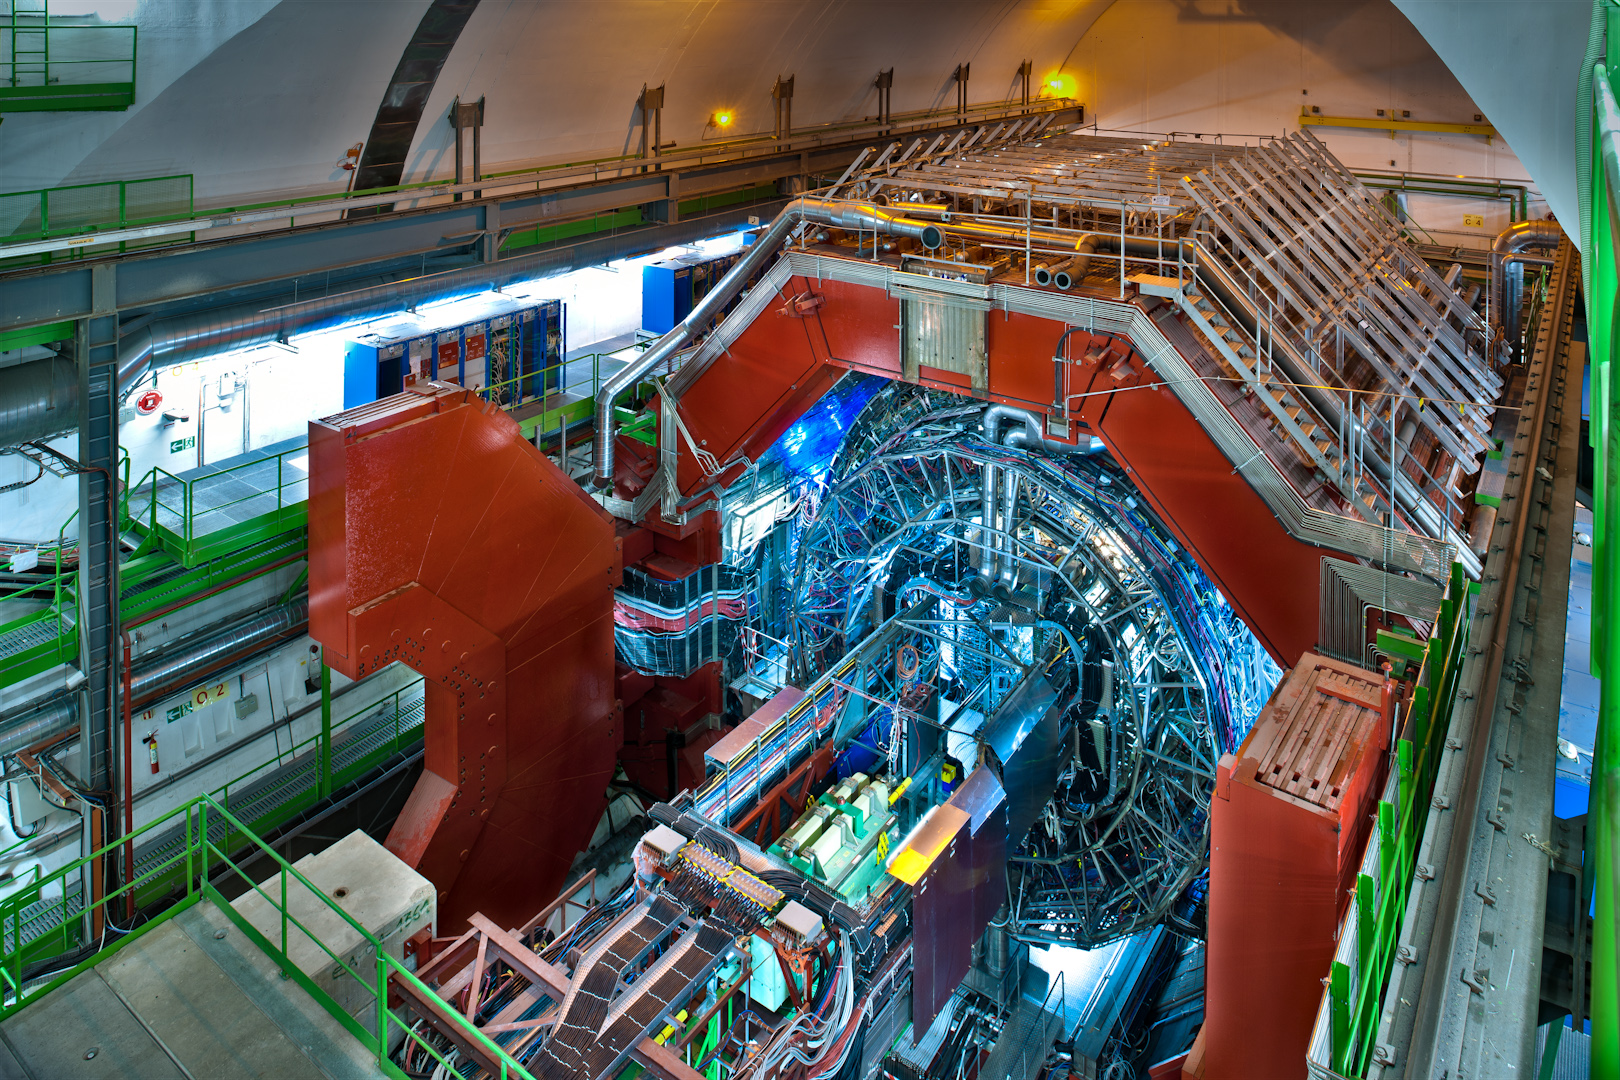
\includegraphics[width=0.6\linewidth]{ALICE/ALICE_LRsaba_CERN_0212_3219.jpg}
        \caption{Foto del rivelatore ALICE}
        \label{fig:ALICEcomplex}
    \end{figure}
    
ALICE \cite{Collaboration_2008_ALICE} è a sua volta composto da vari rivelatori di particelle che permettono di tracciare le traiettorie delle particelle prodotte nella collisione dei fasci, identificarle e misurarne velocità o impulso. I rivelatori di ALICE utilizzati per l'analisi presentata in questa tesi sono descritti nei prossimi paragrafi.

    \subsection{Inner Tracking System (ITS)} \label{ITS}
    L'\textit{Inner Tracking System} è un rivelatore composto da sei cilindri concentrici di rivelatori in silicio di raggio minimo 3.9~cm e massimo 43.0~cm, posizionati con l'asse parallelo alla direzione del fascio. Viene utilizzato per:
    \begin{itemize}
        \item la determinazione della posizione del vertice primario, cioè il punto in cui avviene la collisione dei fasci di protoni; 
        \item la ricostruzione dei vertici secondari di decadimenti di particelle che decadono per interazione debole; 
        \item migliorare la precisione di tracciamento della Time Projection Chamber (TPC) (di cui si parla in seguito nel paragrafo \ref{TPC});
        \item permettere il tracciamento di particelle a basso momento che non vengono tracciate dal rivelatore TPC;
        \item l'identificazione di particelle (PID) con basso impulso trasverso sfruttando la perdita specifica di energia $dE/dx$.
    \end{itemize}
    
    I rivelatori dell'ITS hanno una risoluzione spaziale di poche decine di micrometri. 
    
    \subsection{Time Projection Chamber  (TPC)} \label{TPC}
    La \textit{Time Projection Chamber}  è il principale rivelatore di ALICE per la ricostruzione delle tracce delle particelle prodotte nella collisione. Si tratta di un rivelatore a gas di forma cilindrica, posizionato attorno all'ITS, con raggio interno di 85~cm e esterno di 250~cm e una lunghezza di 500~cm nella direzione del fascio di particelle. Il raggio interno è determinato dalla massima densità di tracce accettabile dalla TPC, quello esterno dalla lunghezza minima necessaria per una precisione del 10$\%$ sulla perdita specifica di energia per ionizzazione $dE/dx$. 
     
     \begin{figure}[htbp]
        \centering
        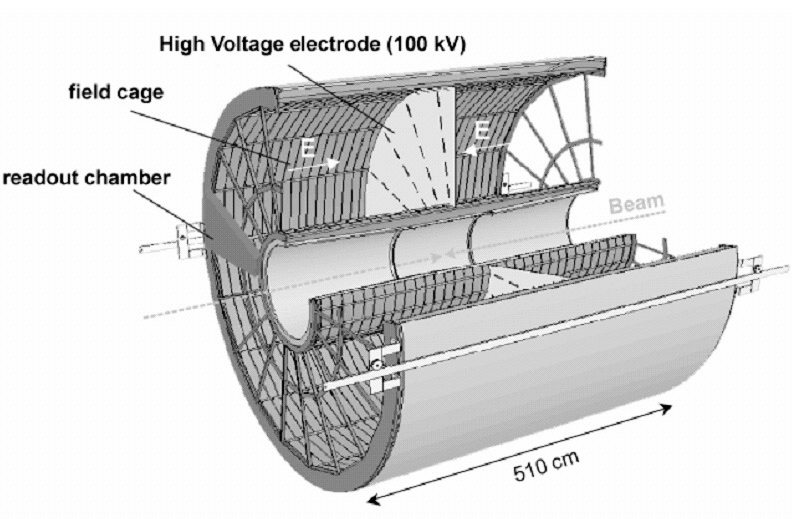
\includegraphics[width=0.7\linewidth]{ALICE/ALICE-TPC-detector.png}
        \caption{Schema della Time Projection Chamber (TPC) di ALICE}
        \label{fig:TPCcomplex}
    \end{figure}
    
    La camera del TPC è riempita con una miscela di gas, che viene ionizzato dal passaggio delle particelle cariche da tracciare. Gli elettroni di ionizzazione vengono accelerati dal campo elettrico creato dagli elettrodi della TPC per arrivare alle placche esterne che permettono di registrare il segnale.
    \\La TPC permette l'identificazione delle particelle tramite la misura della perdita specifica di energia per ionizzazione ($\frac{dE}{dx}$). 
    

    \subsection{Time-Of-Flight (TOF)} \label{TOF}
    Il rivelatore Time-Of-Flight ha forma cilindrica, con raggio minimo di 370 cm e massimo di 399 cm. Questo rivelatore permette l'identificazione delle particelle tramite la misura del tempo di volo dal punto in cui sono state prodotte alla superficie del rivelatore secondo la relazione:
        \begin{equation}
            m = p\sqrt{\frac{t^2_{TOF}}{L^2}-1}
        \end{equation}
    dove $m$ è la massa della particella, $p$ il suo impulso, $t_{TOF}$ il tempo di volo e $L$ la lunghezza della traccia considerata.
    